\chapter{Advanced Tie Points}

%=======================================================================================================
\section{Changing default detector in {\tt  XML\_User/}}


There exist different implemantation of Sift detector and Ann matchor in MicMac. The newest one offer
more option, while the oldest have been more tested \dots 

To change the default behaviour you must edit your {\tt MM-Environment.xml} in the folder {\tt include/XML\_User/}.
For example :



\begin{verbatim}
<MMUserEnvironment>
    <TiePDetect> mm3d:Digeo </TiePDetect>
    <TiePMatch > mm3d:Ann </TiePMatch>
</MMUserEnvironment>
\end{verbatim}

Note that the {\tt mm3d:Digeo} implementation of SIFT detector offers several advantages :

\begin{enumerate}
   \item faster, specially in the gaussian computation;

   \item option {\tt NoMax} and {\tt NoMin}, to supress the Min (or Max) in sift detection,
         this allow to divide by $2$ the number of tie points, while conserving the same ratio
         of multiple tie point (as at $99.99\dots \%$ a max is never a good homolog of a min).
\end{enumerate}



%=======================================================================================================
\section{Filtering tie points in {\tt HomolFilterMasq}}


This command can be used when you have the necessary spatial information to retrieve false
tie points.

The command {\tt HomolFilterMasq} can do some filtering on tie points. The masqing
processe can be purerly in image geometry or can be done in some ground geometry.

\begin{verbatim}
 mm3d HomolFilterMasq
*****************************
*  Help for Elise Arg main  *
*****************************
Mandatory unnamed args : 
  * string :: {Full name (Dir+Pat)}
Named args : 
  * [Name=PostPlan] string :: {Post to plan, Def : toto ->toto_Masq.tif like with SaisieMasq}
  * [Name=GlobalMasq] string :: {Global Masq to add to all image}
  * [Name=KeyCalculMasq] string :: {For tuning masq per image}
  * [Name=KeyEquivNoMasq] string :: {When given if KENM(i1)==KENM(i2), don't masq}
  * [Name=Resol] REAL :: {Sub Resolution for masq storing, Def=10}
  * [Name=ANM] bool :: {Accept no mask, def = true if MasqGlob and false else}
  * [Name=ExpTxt] bool :: {Ascii format for in and out, def=false}
  * [Name=PostIn] string :: {Post for Input dir Hom, Def=}
  * [Name=PostOut] string :: {Post for Output dir Hom, Def=MasqFiltered}
  * [Name=OriMasq3D] string :: {Orientation for Masq 3D}
  * [Name=Masq3D] string :: {File of Masq3D, Def=AperiCloud_${OriMasq3D}.ply}
  * [Name=SelecTer] Pt2dr :: {[Per,Prop] Period of tiling on ground selection, Prop=proporion of selected}
\end{verbatim}

The main option are :

\begin{enumerate}
    \item {\tt PostPlan} for example set {\tt PostPlan=titi} if there is masq per image and for each image 
          {\tt Image.tif} the masq if {\tt Image\_Masqtiti.tif}, by default will generate an error if this
          image does not exist, set {\tt ANM=true} if you know that non existing images are normal;

    \item {\tt GlobalMasq} if masq common to all images exist (for example with fiducial marqs);

    \item {\tt KeyCalculMasq} , sometime you may have many images and a few masq, each masq being applyable
          for a group of images; use this option with much be a computation key desrcibed in
          {\tt MicMac-LocalChantierDescripteur.xml}

    \item {\tt Masq3D} , a file for 3D masq as seized by {\tt SaisieMasqQT}, the orientation {\tt OriMasq3D} 
          must be initialized;

    \item {\tt SelecTer} , can be used to decrease the number of tie points while maintaining the proportion
          of multiplicity;  if {\tt SelecTer=[Per,Prop]}, then in each tile of size $S=Per*Resol$  in the ground coordinate
          \footnote{$Resol$ being the average ground resolution} the point are selected in the subtile of 
          size $S * \sqrt{Prop}$
    
    
\end{enumerate}



%=======================================================================================================

\section{Merging Tie point from multiple view with {\tt HomolMergePDVUnik}}

This command correspond to rather special case, when you have a set of camera that do not move (or form a rigid block) and the scene is moving.
For example :

\begin{itemize}
    \item there is three fixed camera $A,B,C$;
    \item at time $1,2,3,4$ someone is moving in fornt of the camera and the images $A_1,A_2, \dots C_3,C_4$ were acquired ;
\end{itemize}

It is not possible to make some standard photogrammetric processing on $A_1,A_2, \dots C_3,C_4$ as the scene is not static.
By the way if we knew the pose  $P_A,P_B,P_C$ of the camera, then  all the homologous points $(A_1,B_1), (A_2,B_2) \dots (A_4,B_4)$ 
would be compatible witj $P_A$ and $P_B$, which means that we can merge this tie points in a unique file that can be used
to estimate $P_A$ and $P_B$; and the same with $A,C$ and $B,C$. 


The command  {\tt HomolMergePDVUnik} does this merging, in fact you can consider that the tie-points 
obtained are more or less resulting are some kind of merging from the different scene. 

\begin{verbatim}
mm3d HomolMergePDVUnik
*****************************
*  Help for Elise Arg main  *
*****************************
Mandatory unnamed args : 
  * string :: {Full name (Dir+Pat)}
  * string :: {Dir of external point}
Named args : 
  * [Name=PostIn] string :: {Post for Input dir Hom, Def=}
  * [Name=PostOut] string :: {Post for Output dir Hom, Def=MasqFusion}
  * [Name=ExpTxt] bool :: {Ascii format for in and out, def=false}
  * [Name=DirN] vector<std::string> :: {Supplementary dirs 2 merge}
\end{verbatim}



%=======================================================================================================
\section{Tie points on low contrast images usign {\tt SFS} in {\tt MicMac-LocalChantierDescripteur.xml}}


The current implementation of SIFT++ used in MicMac is not fully invariant to scaling/translation in radiometry. This may be a problem in case of acquisitions having a good SNR but with low contrast in the scene; in this case, thanks to good SNR there is potential information to get tie points, but as this information is assimilated to noise, it cannnot be extracted.

To overcome this problem, it is possible to require that MicMac computes some contrast enhancement on images before computing SIFT points. Although this method is not optimal (it would be better to modify the SIFT++ Kernel), it has the advantage of existing\dots



The figure~\ref{FIG:SF:Det} presents an image without enhancement, in its original form, and the same image after enhancement. The figure~\ref{FIG:SF:TieP} presents the detected tie points; we notice that the spatial density of tie points is much higher on enhanced image.

Of course, the enhanced images are fairly artificial, as it can be seen on figure~\ref{FIG:SF:Img} that presents a full image before and after enhancement. So if this option is activated, the enhanced images are used only for the tie points steps (which are developed as specific "hidden files" in folder {\tt Tmp-MM-Dir}).


To activate this option, the {\tt NKS-Assoc-SFS} must be changed in the {\tt MicMac-LocalChantierDescripteur.xml}. It must return {\tt SFS} instead of the default value {\tt NONE}. For example:

\begin{verbatim}
    <KeyedNamesAssociations>
        <Calcs>
            <Arrite>  1 1 </Arrite>
            <Direct>
                <PatternTransform> .* </PatternTransform>
                <CalcName>  SFS </CalcName>
            </Direct>
        </Calcs>
        <Key>   NKS-Assoc-SFS </Key>
    </KeyedNamesAssociations>
\end{verbatim}

\begin{figure}
\begin{center}
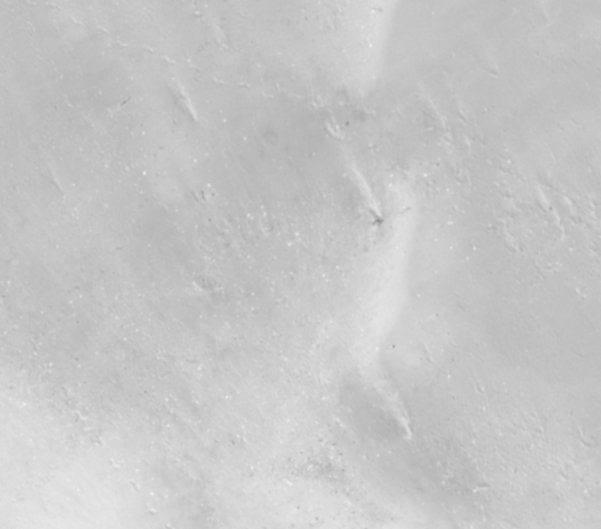
\includegraphics[width=0.4\textwidth]{FIGS/Tapioca-SFS/Detail-STD.jpg}
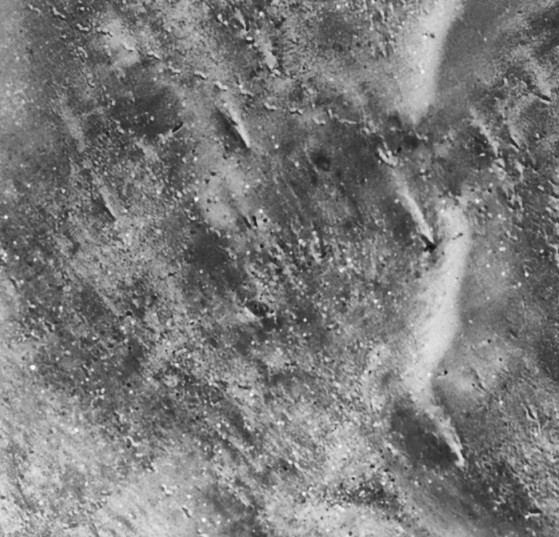
\includegraphics[width=0.4\textwidth]{FIGS/Tapioca-SFS/Detail-SFS.jpg}
\end{center}
\caption{Detail of image before and after enhancement}
\label{FIG:SF:Det}
\end{figure}


\begin{figure}
\begin{center}
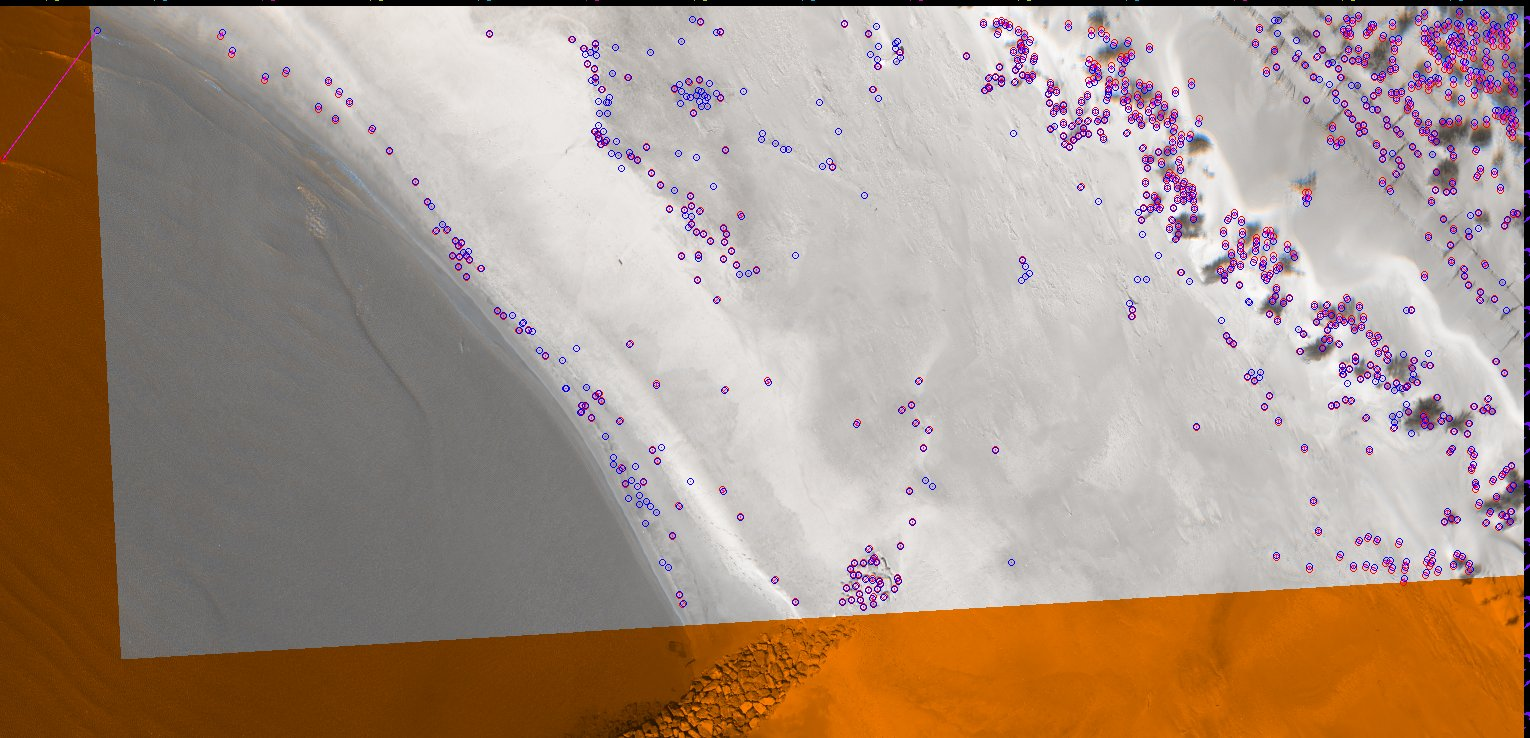
\includegraphics[width=0.95\textwidth]{FIGS/Tapioca-SFS/SIFT-STD.jpg}
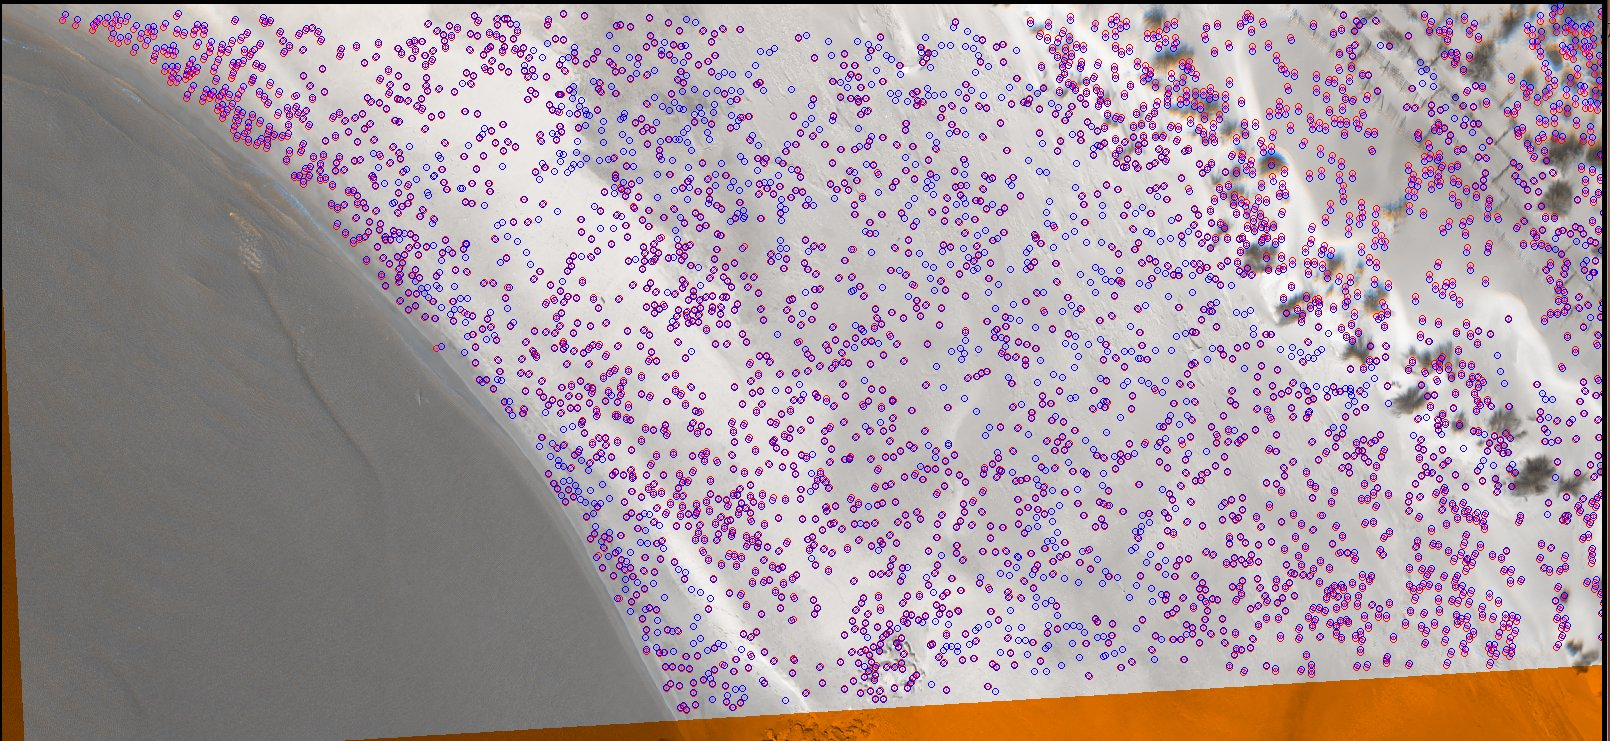
\includegraphics[width=0.95\textwidth]{FIGS/Tapioca-SFS/SIFT-SFS.jpg}
\end{center}
\caption{Tie points before and after enhancement}
\label{FIG:SF:TieP}
\end{figure}

\begin{figure}
\begin{center}
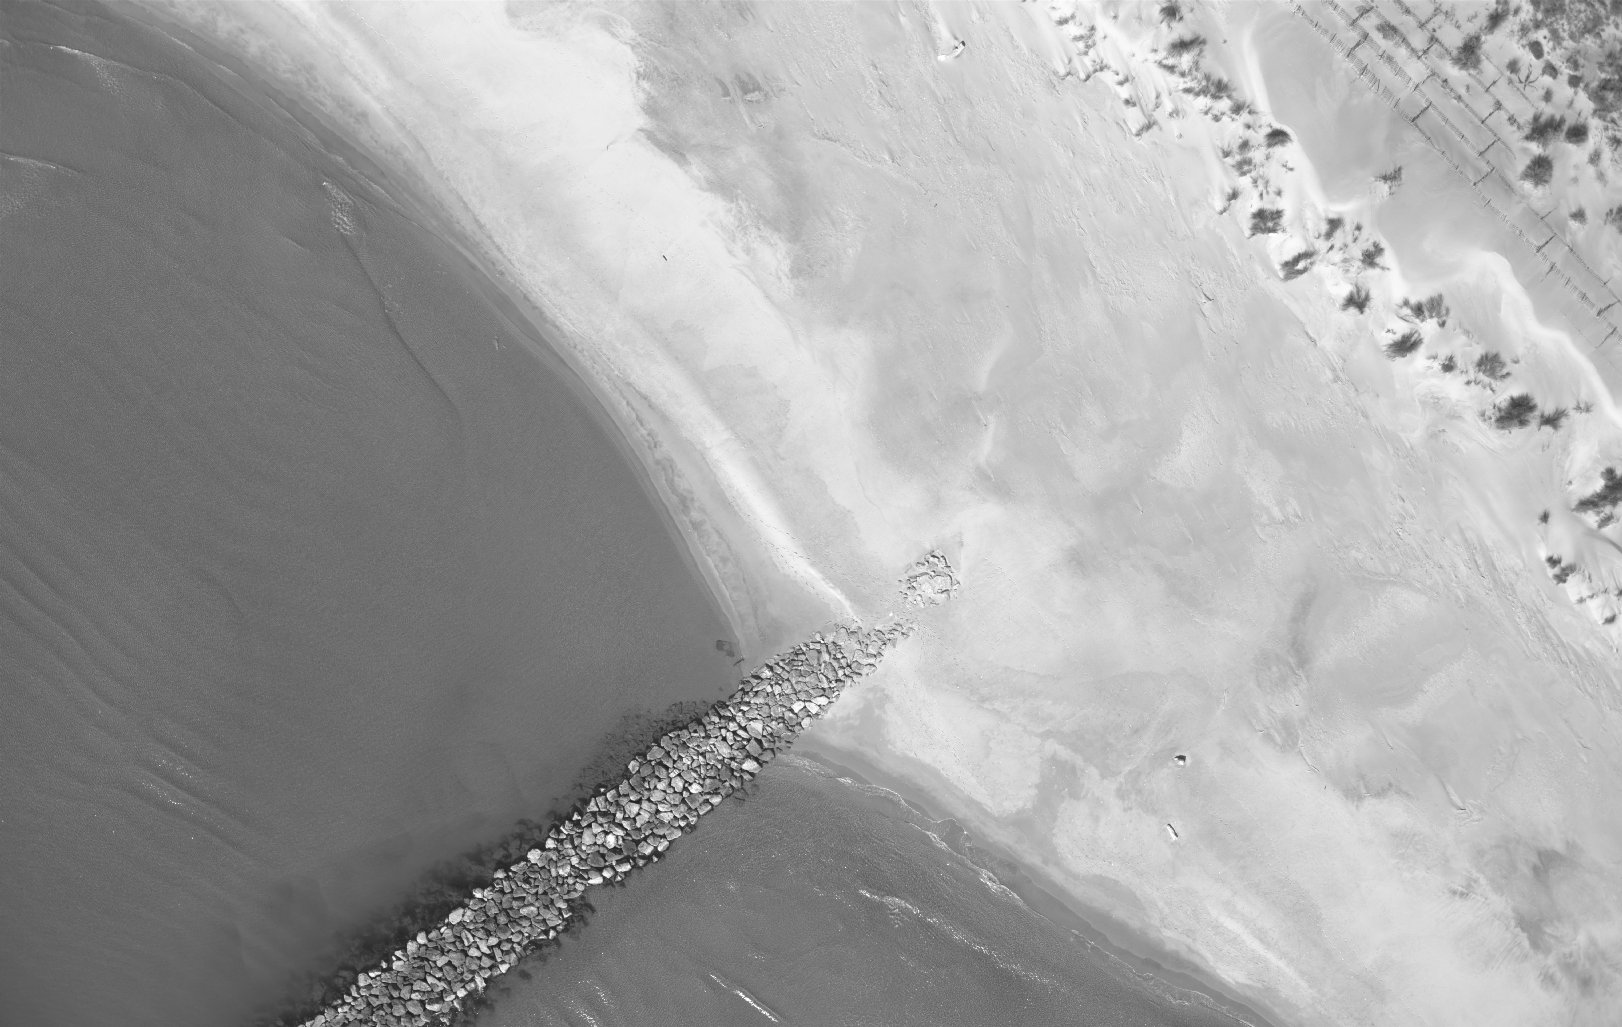
\includegraphics[width=0.95\textwidth]{FIGS/Tapioca-SFS/Im-STD.jpg}

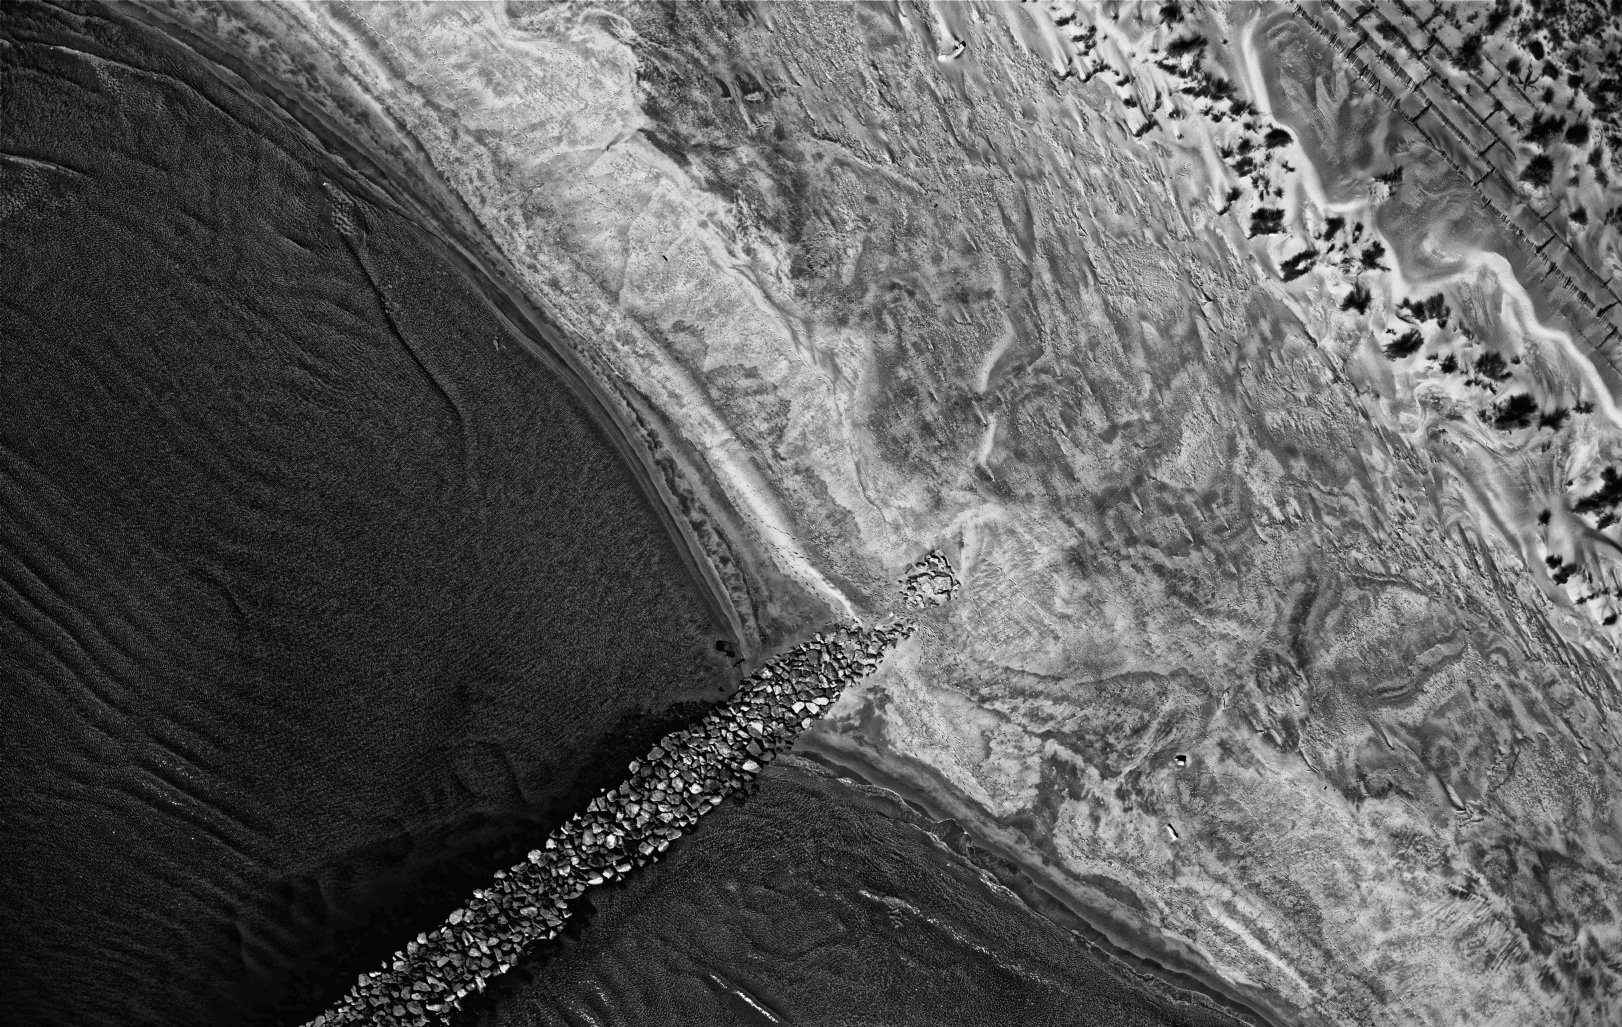
\includegraphics[width=0.95\textwidth]{FIGS/Tapioca-SFS/Im-SFS.jpg}
\end{center}
\caption{Global images before and after enhancement}
\label{FIG:SF:Img}
\end{figure}









